\documentclass[beamer,crop,tikz]{standalone}

\usepackage{formation}
\usetikzlibrary{trees}

\begin{document}
  \begin{tikzpicture}
    \node[inner sep=0pt] (input) at (0,0) {
\includegraphics[width=.25\textwidth]{img/sub-img/ae-denoiser-input.png}};
    \node[hencoder] (noise) at (2, 0) {+};
    \node[inner sep=0pt] (noisy) at (4.1,0) {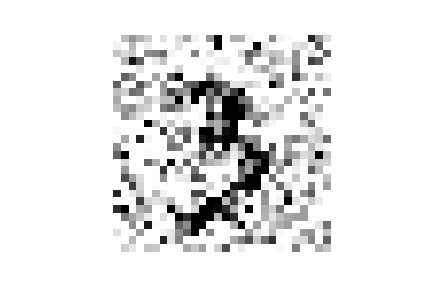
\includegraphics[width=.25\textwidth]{img/sub-img/ae-denoiser-noisy-input.png}};
    \node (legend) at (2, -0.8) {Bruit gaussien};
    \node[hencoder] (encoder) at (6.5, 0) {Encodeur};
    \node[input] (code) at (8.5, 0) {Z};
    \node[output] (decoder) at (10.5, 0) {Décodeur};
    \node[inner sep=0pt] (predict) at (13,0) {
\includegraphics[width=.25\textwidth]{img/sub-img/ae-denoiser-predict.png}};

    \draw[->,>=stealth] ($(input)+(+0.65,0)$) to (noise);
    \draw[->,>=stealth] (noise) to ($(noisy)+(-0.65,0)$);
    \draw[->,>=stealth] ($(noisy)+(0.7,0)$) to (encoder);
    \draw[->,>=stealth] (encoder) to (code);
    \draw[->,>=stealth] (code) to (decoder);
    \draw[->,>=stealth] (decoder) to ($(predict)+(-0.65,0)$);
    
    
  \end{tikzpicture}
\end{document}
